\documentclass[letterpaper]{article}

\usepackage{float}

\usepackage[margin=1in]{geometry} % full-width


% Unicodez, pdf metadata
\usepackage[utf8]{inputenc}
\usepackage{hyperref}
\hypersetup{
	unicode,
%	colorlinks, 
%	breaklinks, 
%	urlcolor=cyan, 
%	linkcolor=blue, 
	pdfauthor={Giovanna G. Amorim, Jonathan Loud, Jacob Rodriguez, Samuel-José Turcotte},
	pdftitle={BIO CE Project - [Title]},
	pdfsubject={},
	pdfkeywords={},
	pdfproducer={Giovanna G. Amorim, Jonathan Loud, Jacob Rodriguez, Samuel Turcotte},
	pdfcreator={Giovanna G. Amorim, Jonathan Loud, Jacob Rodriguez, Samuel Turcotte}
}

%graphics
\usepackage{graphicx}
\graphicspath{ {./figs/} }

%references
\usepackage{biblatex} %Imports biblatex package
\addbibresource{Bio-ce.bib}

%math stuff
\usepackage{algorithm, algpseudocode} % use algorithm and algorithmicx for typesetting algorithms
\usepackage{mathrsfs} % for \mathscr command
\usepackage{amsmath}


%graph stuff
\usepackage{pgfplots}
\pgfplotsset{width=15cm,compat=1.9}

\usepgfplotslibrary{external}
\tikzexternalize


% cover page
\title{On the Laboratory Synthesis of Electric Eel Electrocytes}
\author{Jonathan Loud 2342270, Jacob Rodriguez 2336804, \\
Giovanna G. Amorim 233 4984, Samuel-José Turcotte 2339779}

\date{Dawson College \\[15pt]
000-000-000 section 00001\\[15pt]
Dr. Jeffery K. Eng\\[15pt]
Submission: \today}

\begin{document}

\maketitle

\begin{abstract}
    This paper explores the experimental simulation of electric eel cells. By simulating the electrochemical 
	conditions found within eel electrocytes on a macroscopic scale, this experiment was able to produce 
	significant voltages ranging in the hundreds of millivolts. Specifically, this experiment employed 
	the use of sodium alginate, an organic salt that releases Na+ ions in water, to simulate the release of sodium 
	ions in electrocytes. By using dialysis tubing with a specific pore size, it was possible to trap the alginate 
	while allowing the diffusion of Na+, thereby creating a charge differential across the tubing and inducing a measurable
	voltage.
	\noindent\textbf{Keywords:} [keywords]
\end{abstract}

\tableofcontents

\newpage

\section{Introduction}
\label{sec:introduction}

Native to the freshwater rivers of South America, the \textit{Electrophorus electricus}, or more 
commonly referred to as the electric eel, is known for its ability to generate high voltage shocks,
formally known as electric organ discharges (EOD); these EODs can be classified into low-voltage 
EODs and high-voltage EODs. Low-voltage EODs are expressed at lower frequencies of about 10Hz to
20Hz \parencite{cataniaAstonishingBehaviorElectric2019}, reaching about 10 V \parencite{ElectricCircuits6ElectricEels2015}. 
Therefore, they are more practical for communication and determining the presence of organisms 
in their environment through a process called electrolocation: monitoring 
changes in a particular electric field \parencite{bennettComparativePhysiologyElectric1970}. 
On the other hand, high-voltage EODs are used as an attack or defence mechanism,
the largest recorded voltage discharge being 500V \parencite{ElectricCircuits6ElectricEels2015}.
However, whether the emitted EODs are expressed as low or high 
voltages, they are produced from a specific cell that makes up 80\% of the eel’s body: electrocytes
\parencite{carlsonAnimalBehaviorElectric2015}. These electrocyte cells are arranged in series and 
in parallel and are located in the electric eel’s three most prominent organs: Sach’s organ, the 
Main organ, and Hunter’s organ \parencite{ElectricCircuits6ElectricEels2015}. [cite this figure (Figure 1.)] This 
arrangement allows for the entire eel to be viewed as a battery, with the positive and negative 
poles at the head and tail respectively, allowing for the variety of EOD voltages mentioned above. 
Although electric eels have the potential to release high-voltage EODs, the current produced remains
nonetheless quite minimal (~1 A) \parencite{ElectricCircuits6ElectricEels2015}. This is a result 
of the high resistance of the freshwater where these eels are found, or more precisely, the lack of 
ions to maintain the electric current \parencite{boisseletBiomimeticPotentialElectric2017}. 
Consequently, to optimize the battery potential of the electric eels EOD, research was conducted 
by Lina Guezi \parencite{gueziTheoreticalExaminationConception2023}, a collegue of ours, to produce 
a synthetic replication of the electric eel’s electrocyte 
cells in ionized water. Our experiment aims to test their research findings by making our own battery prototype based off of their work with a few modifications in order to explore 
the potential uses of this biological battery. To do so we used a dialysis membrane to isolate positive sodium ions ( $Na^+$), similarly to how the electric eels do in their
electrocyte cells, which creates a potential gradient across our synthetic electrocyte cell. This process generates a voltage difference 
which then produces an electric discharge. 

\begin{figure}[H]
	\centering
	\includegraphics[width=0.60\textwidth]{fig1.jpg}
	\caption{Electric eel's organ composition (Hunter's organ, the Main organ, and Sach's organ make up 80\% of the eel's organs) with electrocyte cell alignment and polarization.}
	\label{fig:1}
\end{figure}

\section{Material and Methods}
\label{sec:matandmet}

\subsection*{Materials}

\begin{itemize}
	\item Drinking glasses or other receptacles capable of holding water
	\item Dialysis tubing with a MWCO of 6-8kDa
	\item Sodium alginate powder
	\item Voltmeter
	\item Alligator wires
\end{itemize}

\subsection*{Method}

\begin{enumerate}
	\item Drinking glasses were rinsed and filled with hot tap water. Roughly 10cm pieces of dialysis tubing were cut, and one piece of tubing was soaked in each glass for 30 minutes.
	\item Dialysis tubing pieces were removed from the water, opened up, and a knot was tied at the bottom of each piece, sealing it. 1.25mL of sodium alginate powder was inserted into each section of tubing, and the tubes were filled around 3/4 of the way with water to dissolve the powder. Stirring rods were used to aid soaking and dissolution of the powder.
	\item The filled dialysis membranes were placed back into their glasses, open side up, ensuring that the top of each piece protruded past the water level in the glasses.
	\item The setup was left for 12 hours to maximize ionic diffusion.
	\item The voltage of each sample was measured by placing two alligator-clip wires in each glass: one wire was placed inside the dialysis tubing, and one was placed in the glass but outside the tubing. The positive probe of the voltmeter was then attached to the wire outside the tubing, and the negative probe was connected to the wire inside the tubing. A reading was then made using the voltmeter and the data was recorded. This was repeated for each replicate.
\end{enumerate}

\begin{figure}[h]
	\centering
	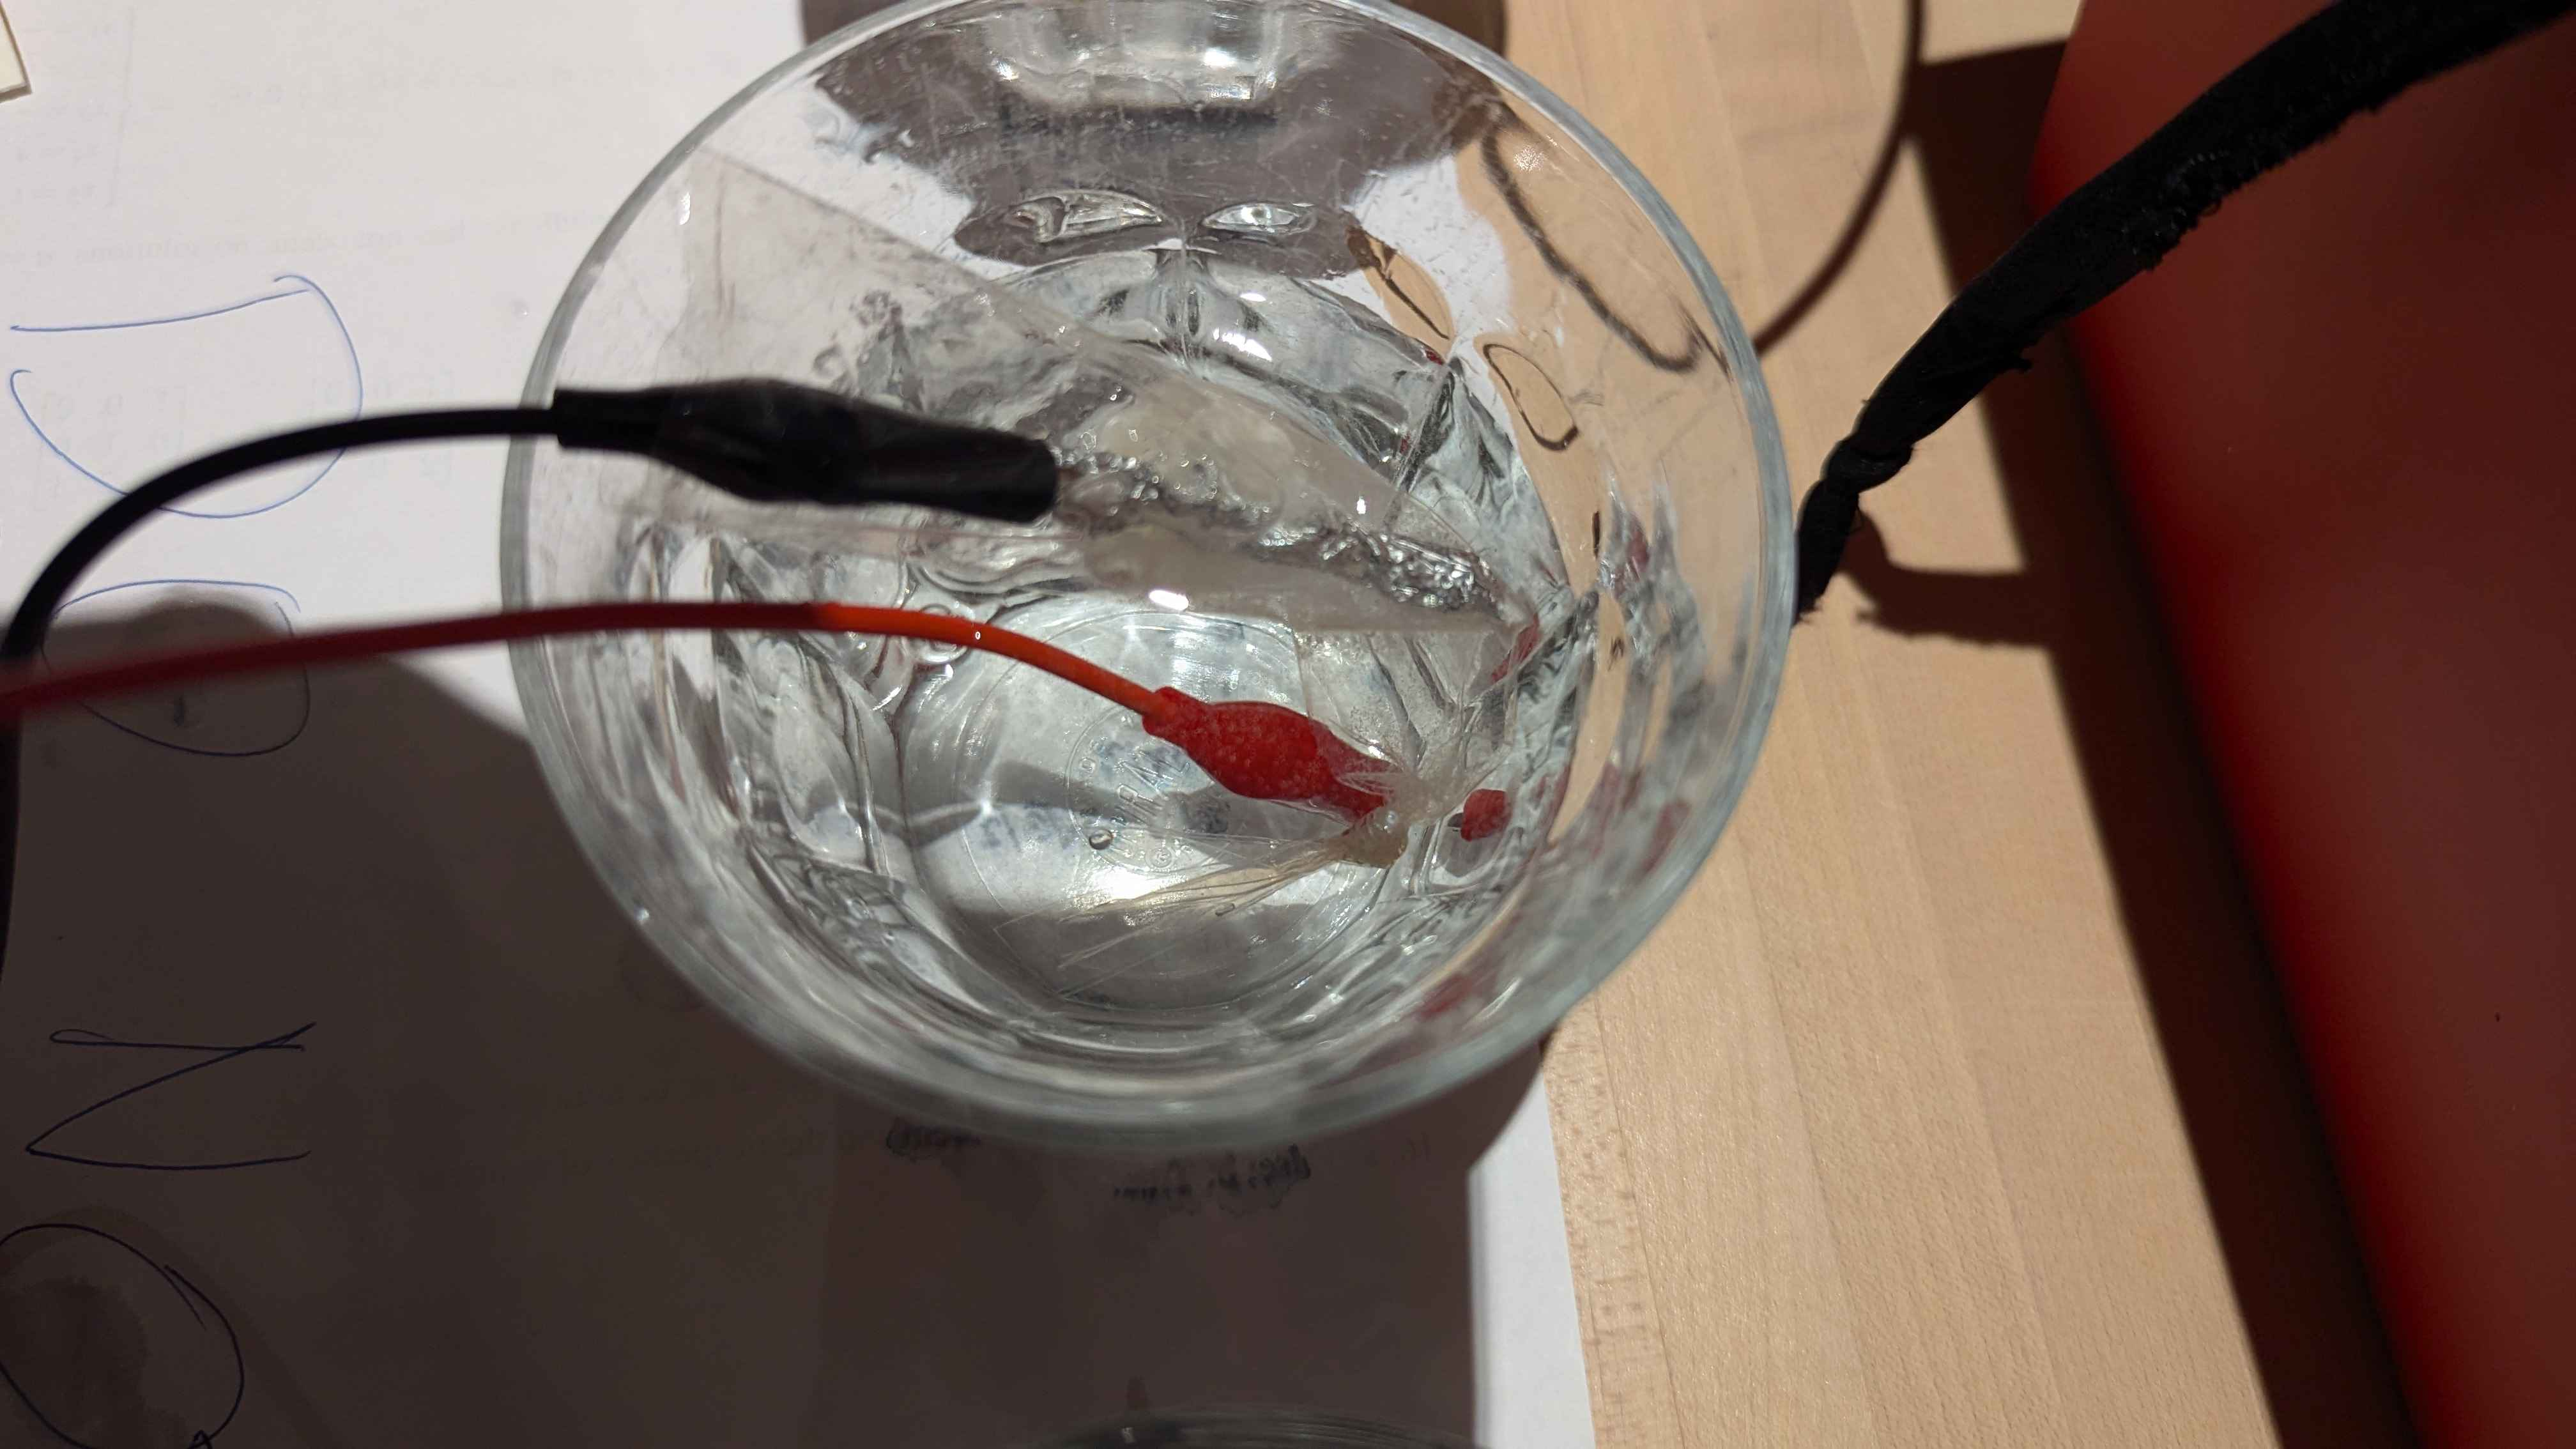
\includegraphics[width=0.60\textwidth]{fig2.png}
	\caption{Experiment with aluminium foil attached to electrode}
	\label{fig:2}
\end{figure}

\begin{figure}[h]
	\centering
	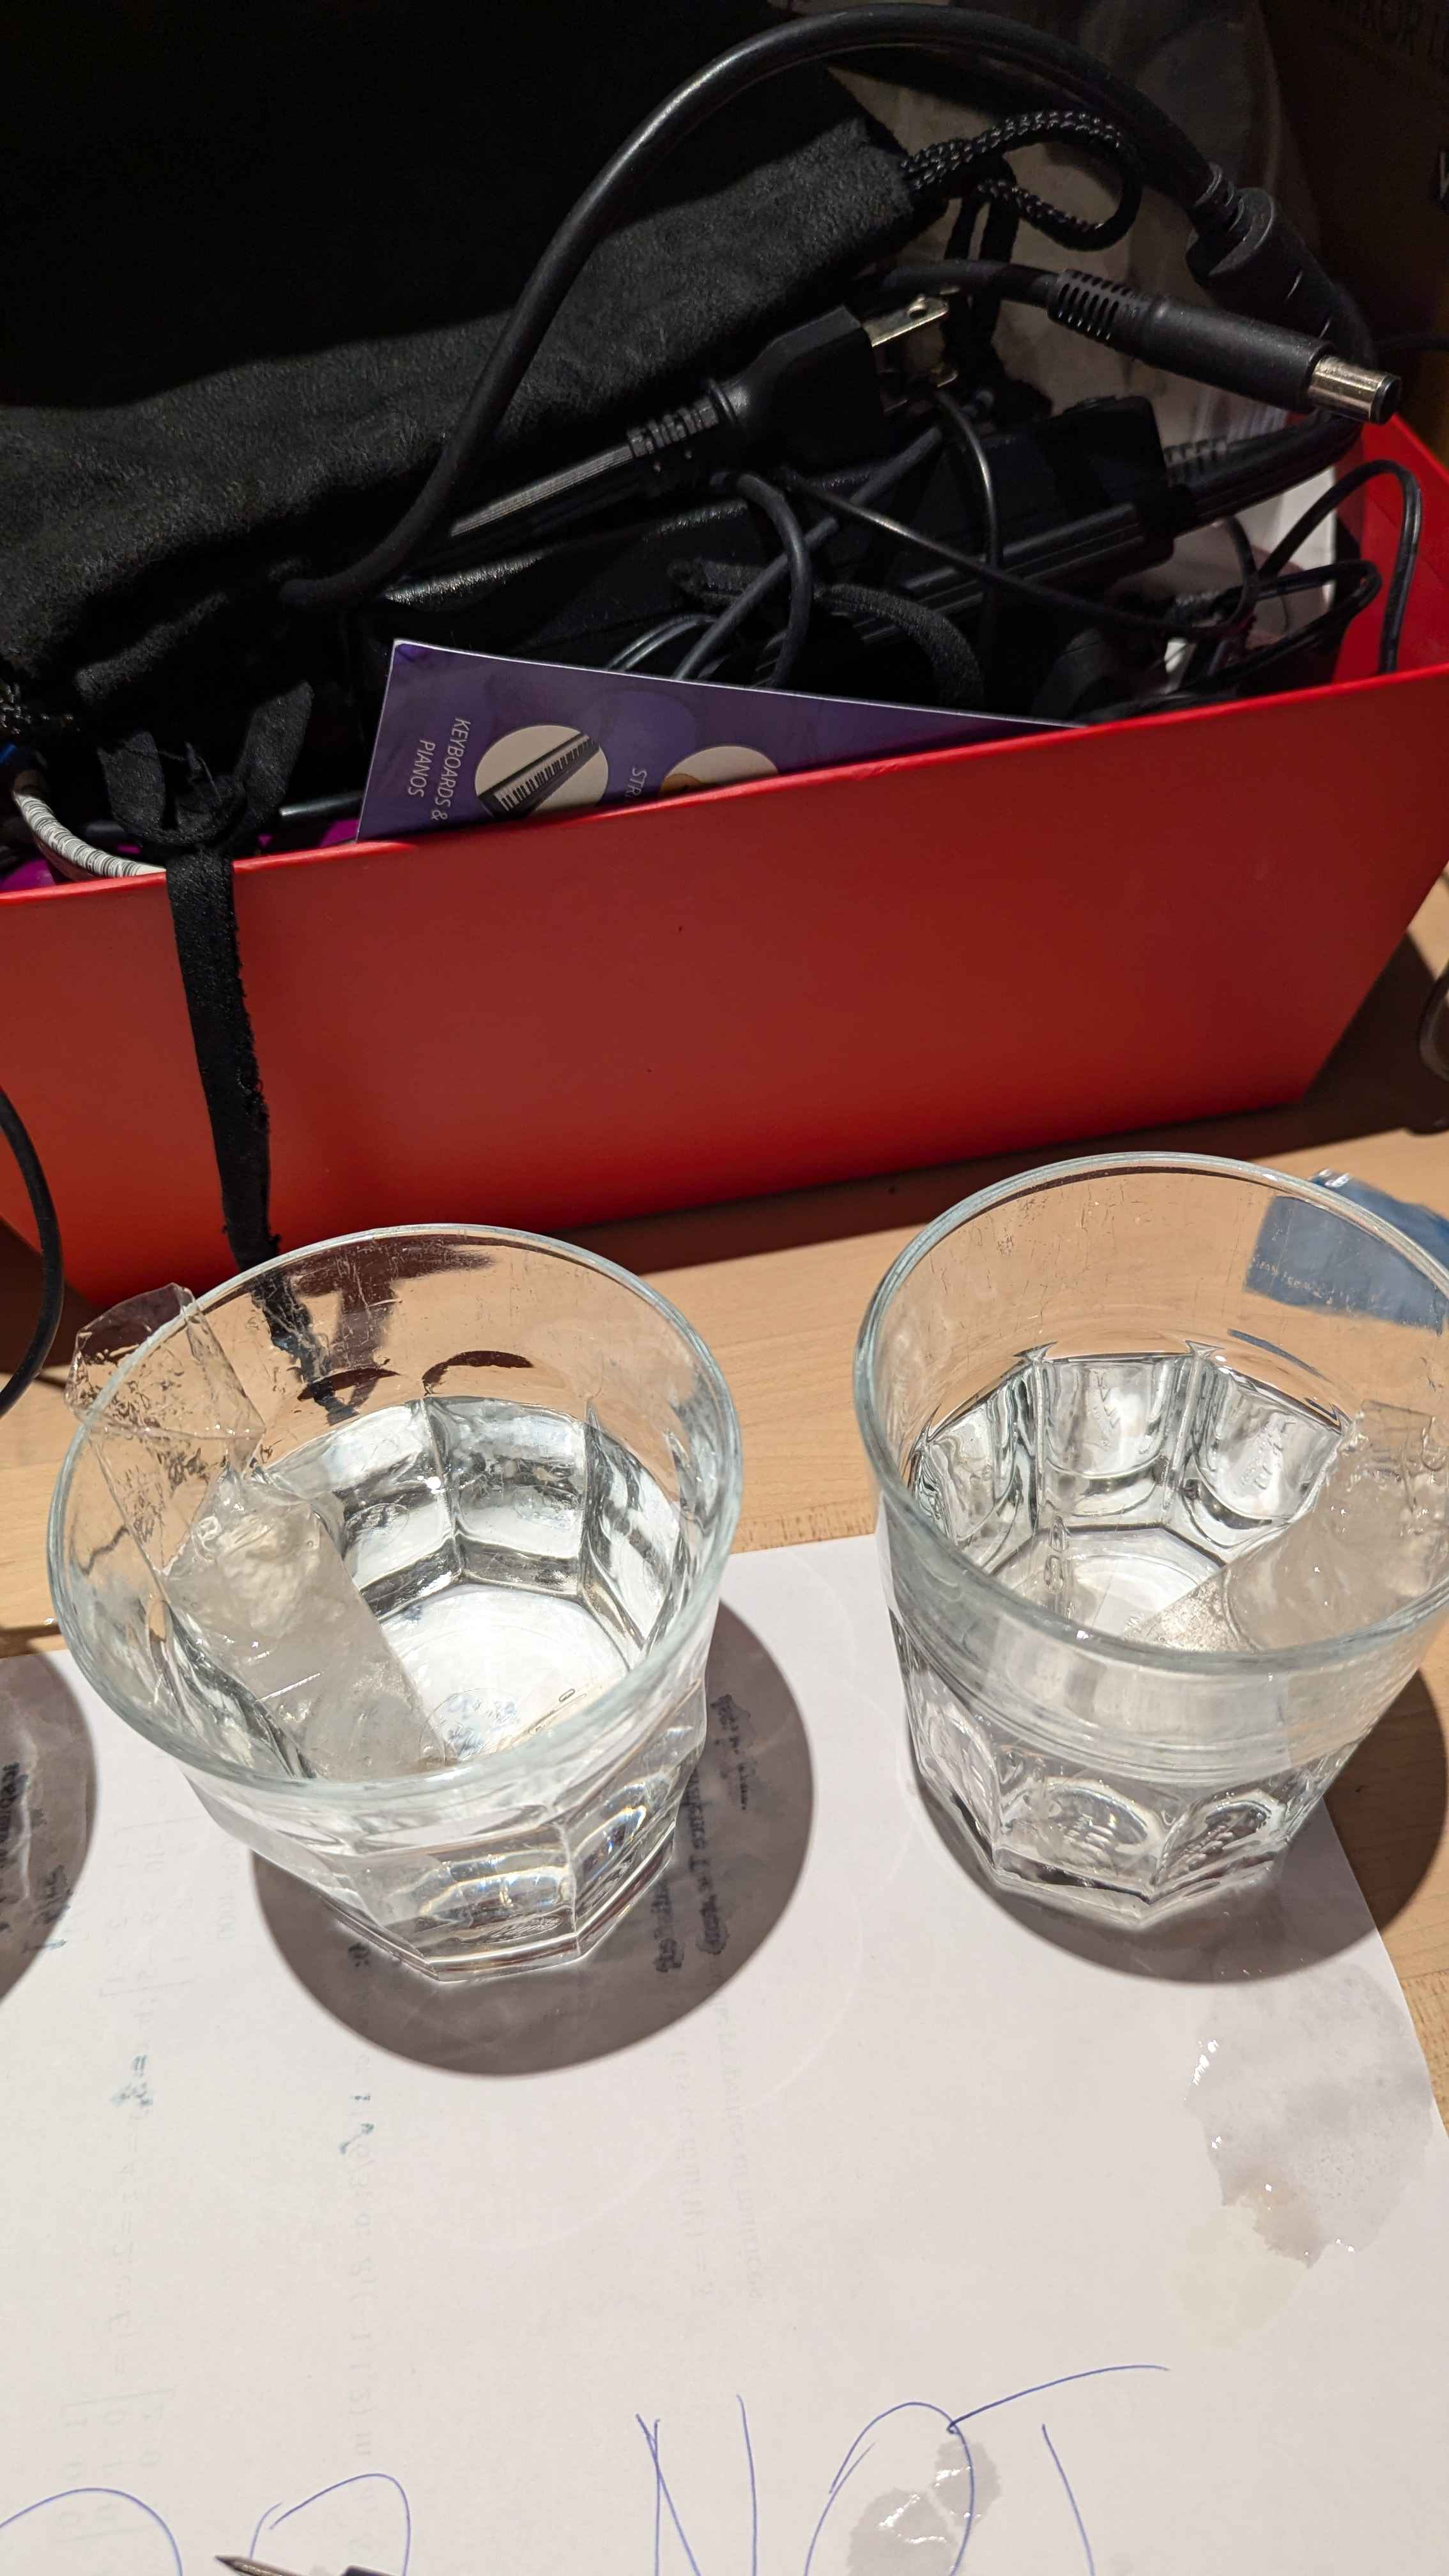
\includegraphics[width=0.60\textwidth]{fig3.png}
	\caption{Membranes being left to diffuse}
	\label{fig:3}
\end{figure}

\section{Results and Discussion}
\label{sec:results and Discussion}





\printbibliography[heading=bibintoc]

\end{document}

